\section{Roboterarchitektur und Systemkomponenten}
\label{sec:roboterarchitektur-und-systemkomponenten}

Folgendes Kapitel beschreibt den physischen Aufbau des \gls{go1} und die Konfiguration dessen im Werkszustand.
Um die Komplexität des Systems besser verstehen zu können, wird der Aufbau in mehreren Schritten erklärt.
Zuerst soll der äußere Aufbau dargestellt werden, danach der Aufbau der internen Systemelemente und der Sensorik und zuletzt
soll die Inbetriebnahme und vereinfachte Nutzung des Roboters dokumentiert werden.


\subsection{Aufbau}
\label{subsec:aufbau}

Im Folgenden soll die interne Architektur des \gls{go1} im Detail dargestellt werden.
Hierfür werden einige Perspektiven des Roboters gezeigt, um die nach Einsatzzweck klassifizierten Bauteilgruppen zu erläutern und darzustellen.

\subsubsection{Überblick}

Die zoomorphe Form des \gls{go1} ist - wie bereits mehrfach angedeutet - an die eines Hundes angelehnt.
So ergeben sich die Bezeichnungen der äußerlich erkennbaren Bauteile von selbst.
Abbildung~\ref{fig:allgemeine_architektur} zeigt die äußerlichen Merkmale im Überblick.

\begin{figure}[h]
    \frame{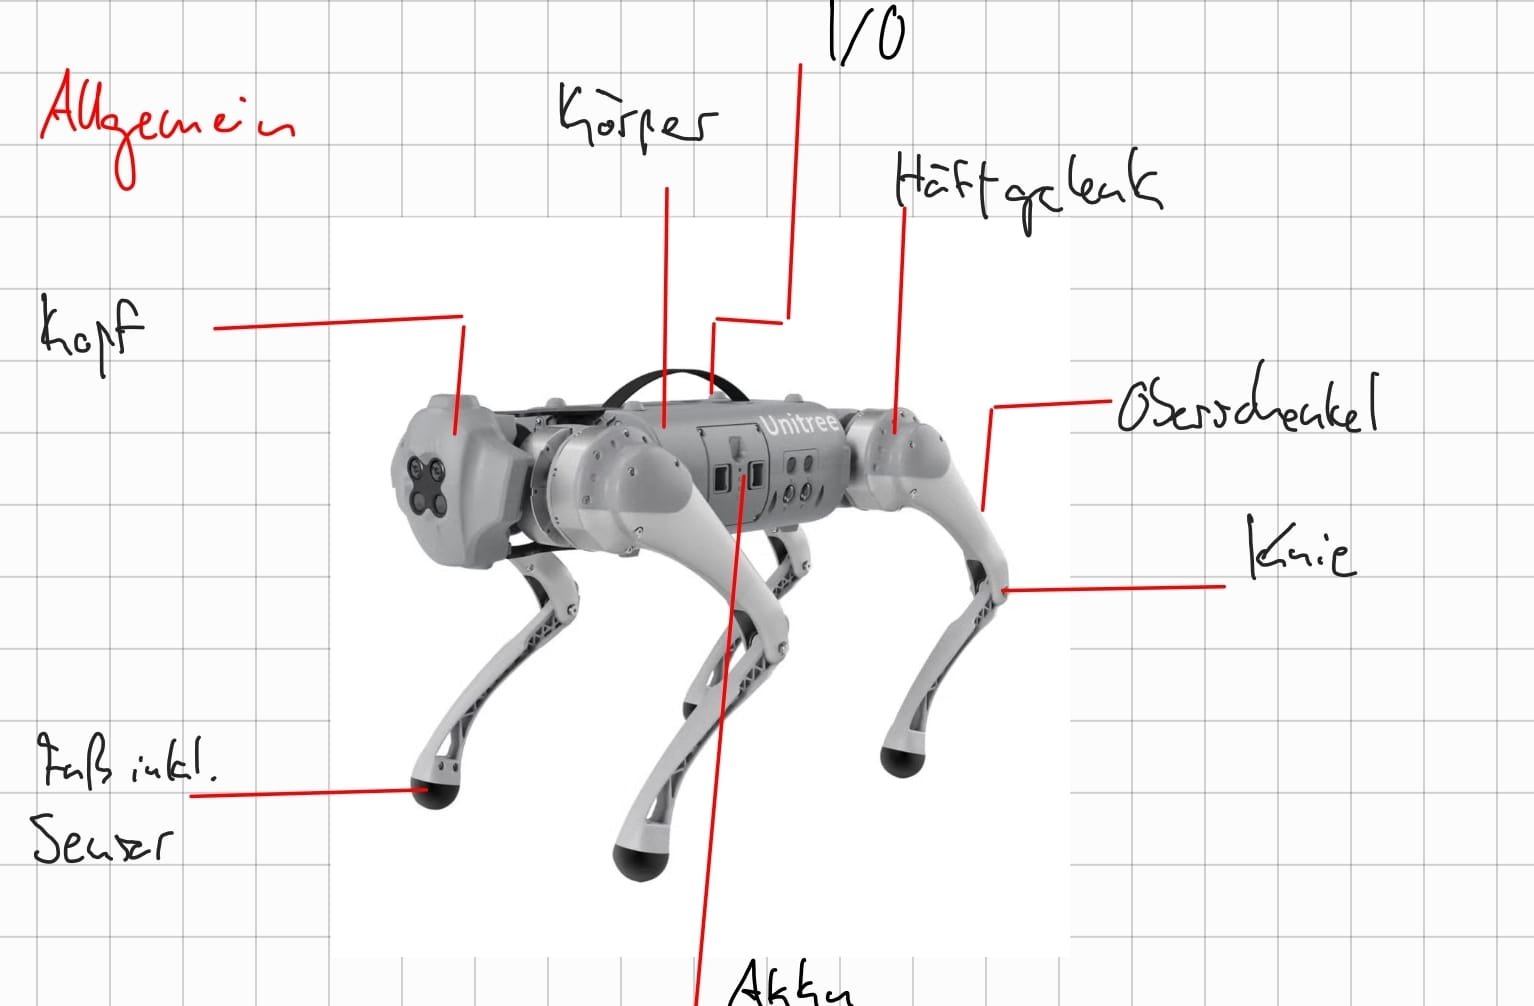
\includegraphics[width=\linewidth]{img/architektur/allgemein}}
    \caption{Überblick über den \gls{go1}}\label{fig:allgemeine_architektur}
\end{figure}

Die Grundlage des Roboters bildet der Körper - auf Abbildung~\ref{fig:allgemeine_architektur} mit \numref{1} gekennzeichnet.
In diesem sind ie meisten Komponenten des \gls{go1} verbaut, unter Anderen die folgenden:
\begin{itemize}
    \item Interne Hardwarekomponenten
    \item Intelligenter Akku
    \item Teile der Sensorik und Kameras
    \item Hüftgelenke und Motoren der Beine
\end{itemize}
Eine genauere Beschreibung der Einzelteile findet sich in den folgenden Unterkapiteln.
An der Vorderseite des Körpers ist der Kopf \numref{2} des Roboters verbaut.
In diesem sind beispielsweise ein \emph{Nvidia Jetson Nano}, eine Stereo-Kamera und Stereo Ultraschall Sensoren
und weitere Bauteile wie Lautsprecher und Mikrofone verbaut.
An den vier äußeren Ecken des Körpers sind die Beine des Roboters verbaut.
Innerhalb des Körpers sind die Motoren zur Steuerung der Hüftgelenke \numref{3} integriert.
Außerhalb der Hüftgelenke an der Oberseite der vier Oberschenkel \numref{4} sind vier weitere Motoren
zur vertikalen Steuerung der Beine verbaut.
Parallel zu diesen Motoren sind im äußeren Teil des oberen Oberschenkels identische Motoren
zur Steuerung der Knie \numref{5} integriert, die die Gelenke jeweils durch steife Achsen und Seilzüge
anwinkeln können.
An den Enden der Beine sind jeweils Füße \numref{6} verbaut, in denen Drucksensoren integriert sind.

Neben den äußerlich auffälligen Merkmalen ist auf der linken Seite des Körpers noch ein intelligenter Akku
\numref{7} verbaut.
Auf der Oberseite des Körpers sind unterhalb der Tragevorrichtung \numref{8} noch Schnittstellen \numref{9} zur physischen
Verbindung auf die integrierten Hardwarekomponenten verbaut.

% ----- Ende ----------
% ----- Überblick -----

\subsubsection{Mechanische Komponenten}

Der Anteil der in Abbildung~\ref{fig:mechanische_komponenten} gezeigten mechanischen Elemente des \gls{go1} hält sich in Grenzen.
So sind am Körper selbst lediglich vier bewegliche Teile angebaut - die vier Servomotoren
der Hüftgelenke \numref{1}.
An den Hüftgelenken befestigt sind die einzigen weiteren beweglichen Bauteile des Roboters,
die pro Bein jeweils zwei weiteren Motoren für die Neigung der Beine \numref{2} und der Kniegelenke \numref{3}.
\todo{Validieren ob starre und Seizug Verbindung genutzt werden}
\begin{figure}[h]
    \frame{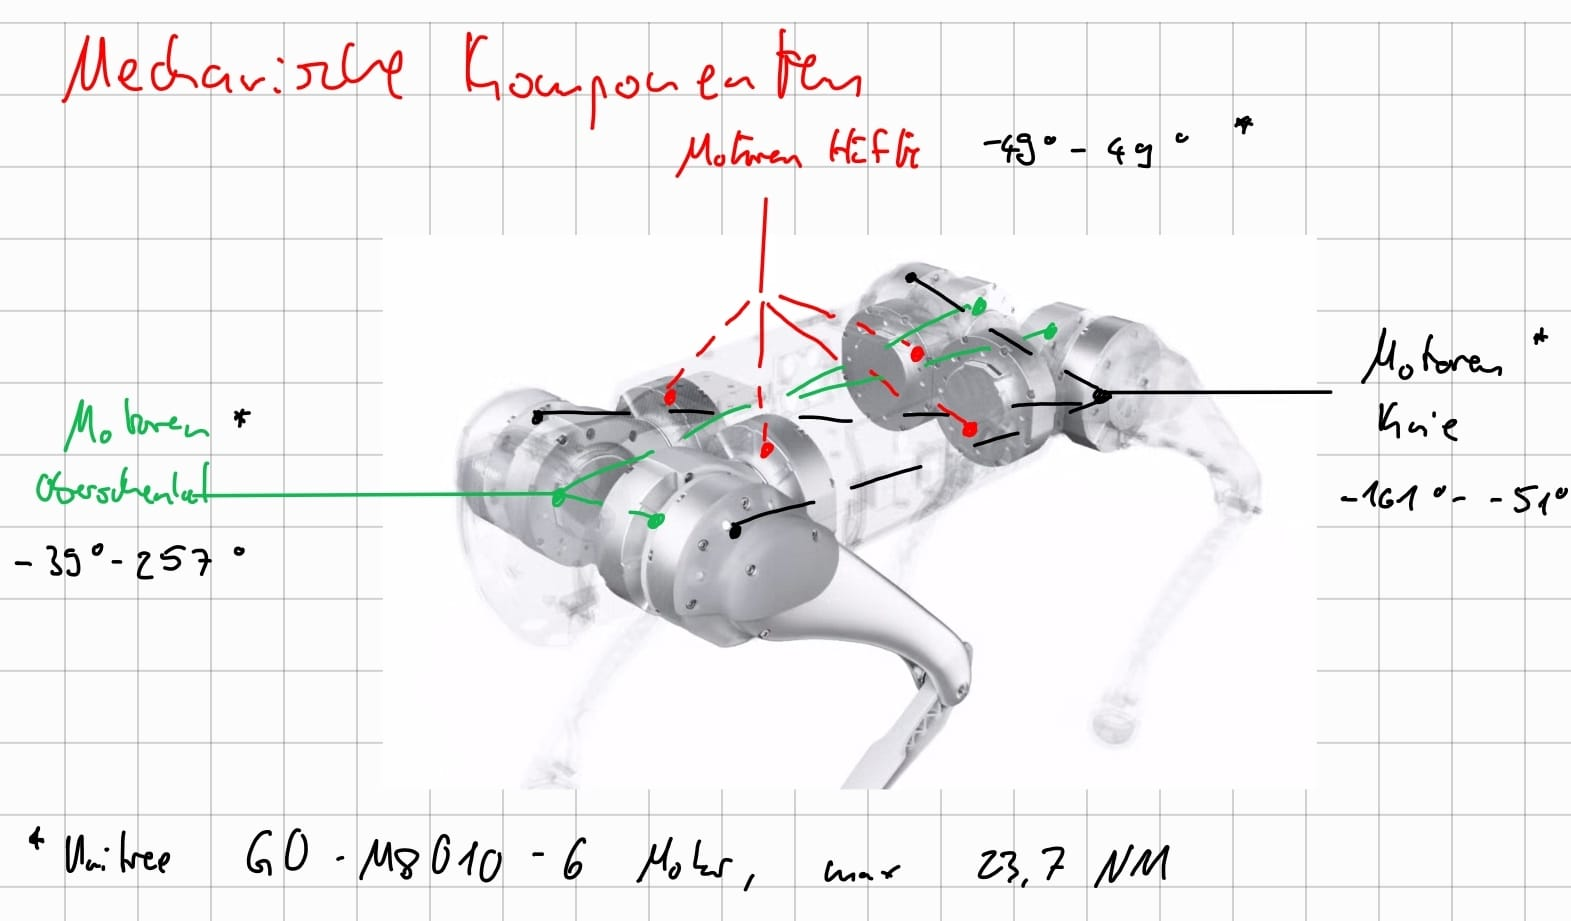
\includegraphics[width=\linewidth]{img/architektur/mechanische_komponenten}}
    \caption{Mechanische Komponenten des \gls{go1}}\label{fig:mechanische_komponenten}
\end{figure}
Zum Strecken des Kniegelenks wird eine am äußeren Motor angebrachter Seilzug \numref{4} verwendet,
zum Anwinkeln des unteren Beines wir im Gegenzug eine starre Verbindung \numref{5} an der Vorderseite des Kniegelenks genutzt.

\myparagraph{Eigenschaften der Servomotoren}
Die Servomotoren am Hüftgelenk - Abbildung~\ref{fig:mechanische_komponenten}, Bauteil \numref{1}, die Motoren an den Beininnenseiten \numref{2}
und die Motoren an den Beinaußenseiten \numref{3} sind des gleichen Models -
\emph{Unitree Robotics GO-M8010-6 Motor}\footcite{go_motor}.
Die Servomotoren \todo{Sicher Servo?} haben ein maximales Drehmoment von \num{23.7}\gls{nm} und können in 3 verschiedene Konfigurationen
eingeteilt werden:
\begin{enumerate}
    \item \textbf{Hüftmotoren}\\
    Bewegungsradius von \num{-49}\textdegree~bis \num{49}\textdegree
    \item \textbf{Oberschenkelmotoren}\\
    Bewegungsradius von \num{-39}\textdegree~bis \num{257}\textdegree
    \item \textbf{Kniemotoren}\\
    Bewegungsradius von \num{-161}\textdegree~bis \num{-51}\textdegree
\end{enumerate}
Die Motoren sind ebenfalls mit Sensorik bestückt, welche den aktuellen Zustand des Bauteils erkennen und
an die \gls{mcu} schicken können.
Diese Funktionalität wird im Kapitel~\ref{subsubsec:hardware_sensorik} näher beschrieben.

\subsubsection{Hardware und Sensorik}
\label{subsubsec:hardware_sensorik}

Als wichtige Bausteine zur intelligenten Nutzung des \gls{go1} sind an vielen Stellen im Roboter
einige Sensoren oder intelligente Hardware verbaut.
Neben der dedizierten Sensorik zur Erkennung des Umfeldes ist ebenfalls einfachere Sensorik
in einigen Bauteilen wie den mechanischen Bauteilen des Laufapparats verbaut.
Abbildung~\ref{fig:laufapparat} zeigt die hierfür verbauten Sensoren und intelligenten Hardwarebausteine.

\begin{figure}[h]
    \frame{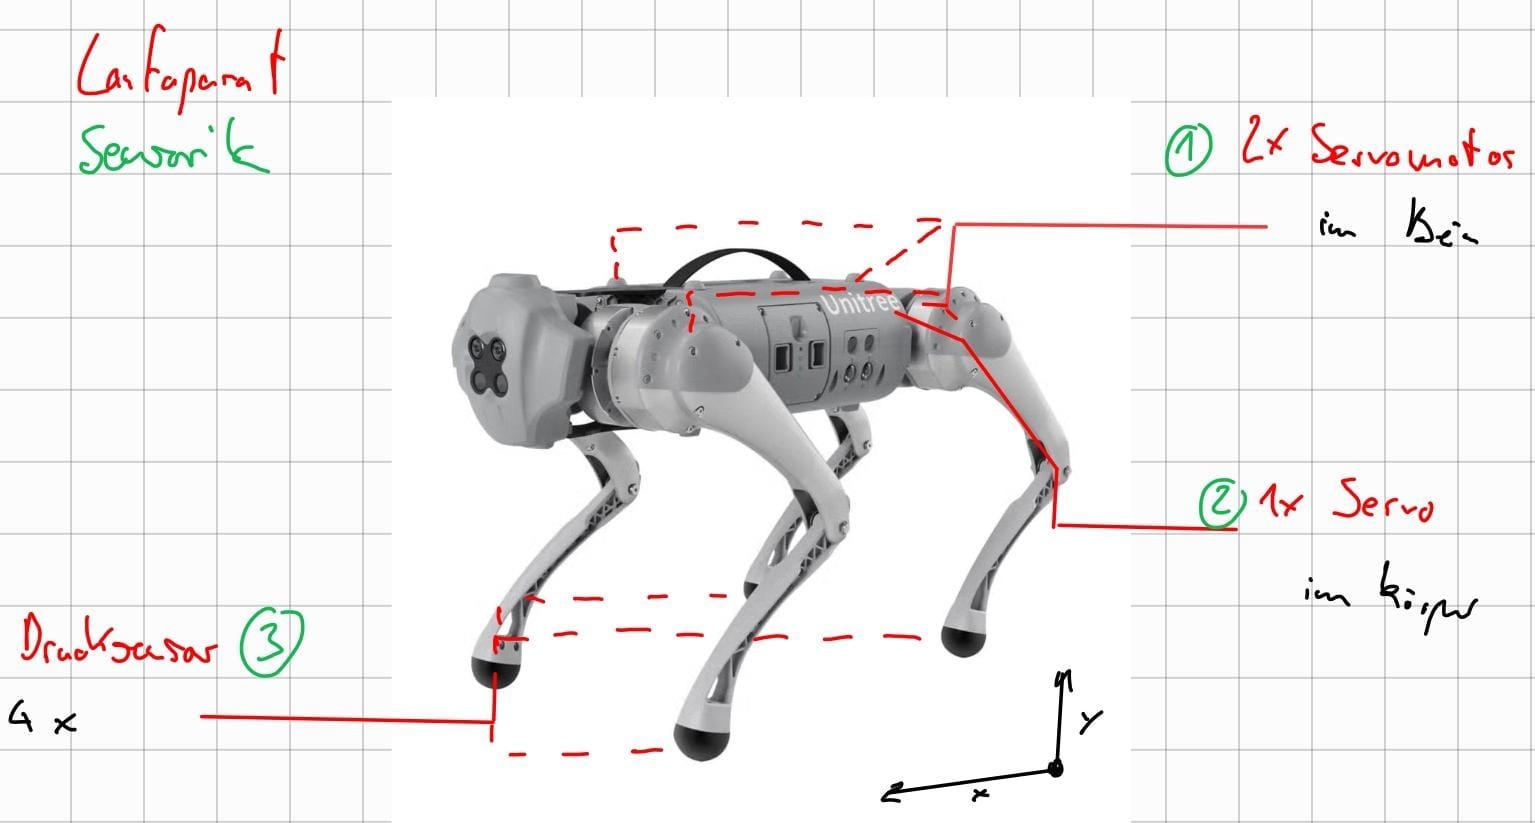
\includegraphics[width=\linewidth]{img/architektur/laufaparat}}
    \caption{Sensorik und Daten des Laufaparats}\label{fig:laufapparat}
\end{figure}

Ähnlich der mechanischen Eigenschaften der zwölf Servomotoren des Typs \emph{GO-M8010-6} - zwei pro Bein des Roboters \numref{1}
und je ein Motor im Körper des Roboters \numref{2} - sind die sensorischen Funktionen dieser identisch.
In Abbildung~\ref{fig:netzwerk_ueberblick} in Kapitel~\ref{subsubsec:netzwerk_ueberblick} ist erkennbar, dass die
zwölf Motoren des \gls{go1} über eine \emph{RS-485} Schnittstelle mit der \gls{mcu} verbunden sind.
Diese wertet die Informationen aus und steuert die einzelnen Motoren über dieselbe Schnittstelle an.

\begin{figure}[h]
    \frame{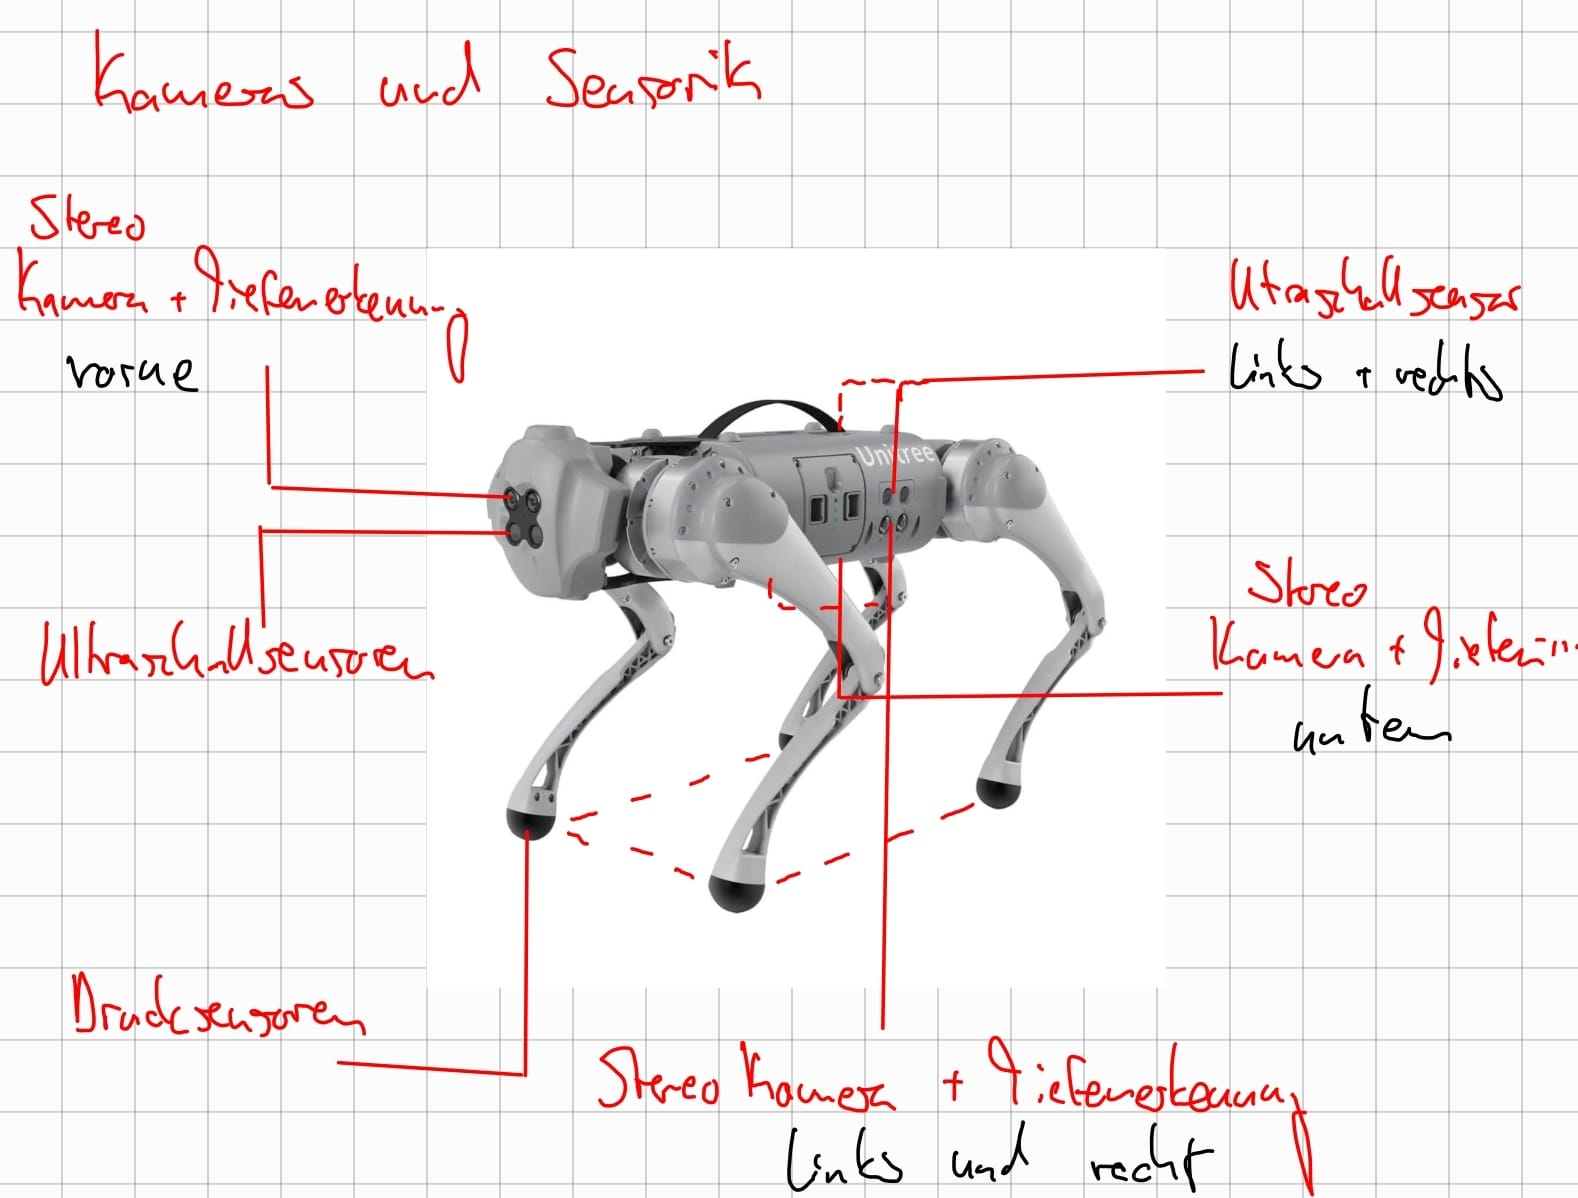
\includegraphics[width=\linewidth]{img/architektur/kameras_sensorik}}
    \caption{Darrstellung der verbauten Kamera und Sensorik}\label{fig:kameras_sensorik}
\end{figure}

\begin{figure}[h]
    \frame{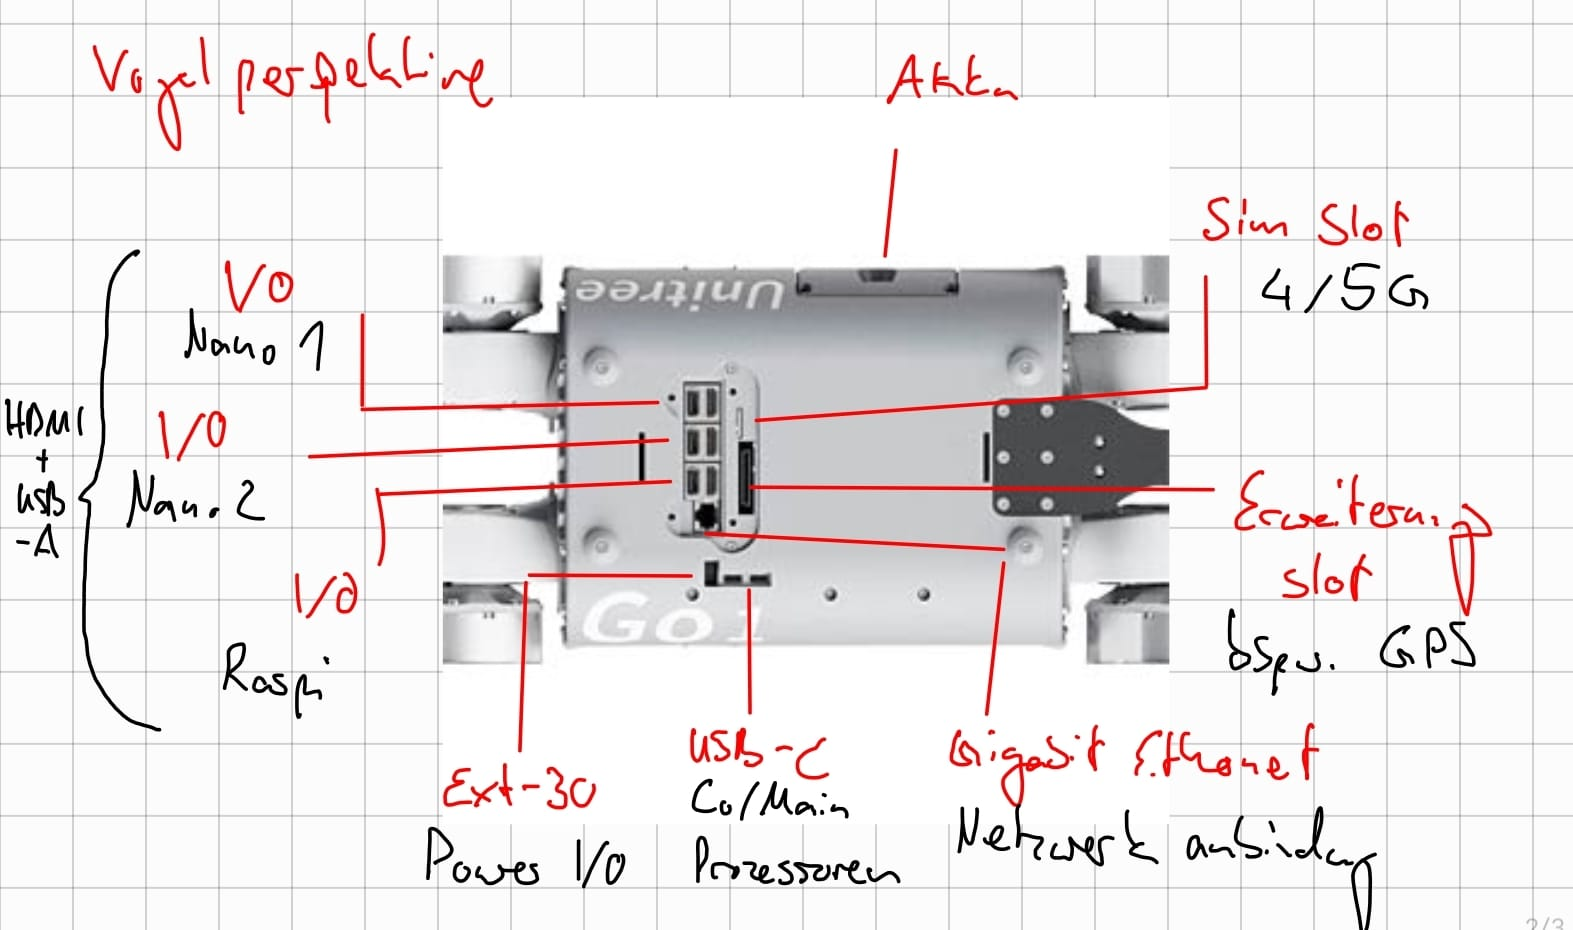
\includegraphics[width=\linewidth]{img/architektur/hardware}}
    \caption{Vogelperspektive mit Hardware}\label{fig:hardware}
\end{figure}


\subsection{Inbetriebnahme}
\label{subsec:inbetriebnahme}

In diesem Kapitel wird die erste Inbetriebnahme des Roboters beschrieben.
Hierzu werden auch die Inhalte und Erweiterungen aufgelistet, welche im Lieferumfang für einen \gls{go1} Edu enthalten sind.
Anschließend soll der Betrieb durch den Akku und ein Netzteil beschrieben werden.

% todo an aus fernbedienung?

\subsubsection{Lieferumfang}

Abbildung \ref{fig:lieferumfang} zeigt die im Lieferumfang enthaltene Transportbox aus Styropor und deren Inhalte, welche
gleichzeitig der gesamte Lieferumfang des \gls{go1} in der \emph{Edu} Version ist.

\begin{figure}[h]
    \frame{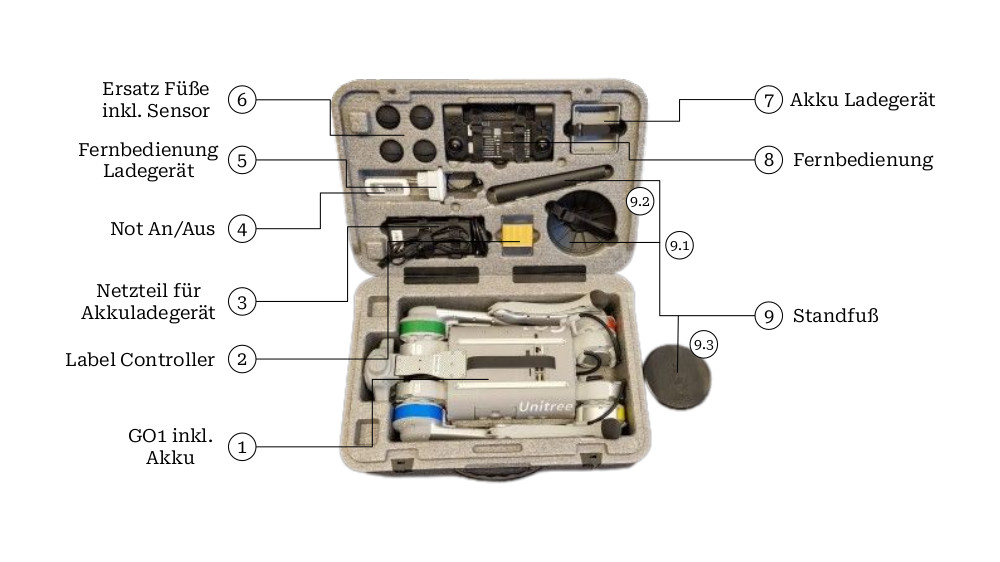
\includegraphics[width=\linewidth]{img/analyse/lieferumfang}}
    \caption{Ansicht der Transportbox und des Lieferumfangs}\label{fig:lieferumfang}
\end{figure}

\noindent Im Lieferumfang enthalten sind folgende Elemente:

\begin{enumerate}
    \item \gls{go1} inklusive Akku
    \item Kompakte Fernbedienung mit \emph{Folge-Mir}-Funktion
    \item Netzteil für das Akku-Ladegerät
    \item Fernbedienung für An-/Ausschaltfunktion
    \item Ladegerät für die Fernbedienungen inklusive \gls{usb}-A auf \gls{usb}-C Kabel
    \item Vier Ersatzfüße inklusive der integrierten Drucksensoren
    \item Akku-Ladegerät mit \gls{usb}-C Anschluss zur Akkuinspektion
    \item Fernbedienung
    \item Standfuß aus drei Teilen für die Ablage des \gls{go1}
    \begin{enumerate}
        \item Sockel
        \item Verlängerung
        \item Plattform inklusive Einkerbungen zum Ausbalancieren des aufliegenden \gls{go1}
    \end{enumerate}
\end{enumerate}

Sollte kein weiteres Zubehör konfiguriert sein, so sind an den Montagestellen auf der Oberseite des Roboters Gummienden
zum Schutz des Korpus bei Rotationen montiert.
Je nach bestelltem Zubehör - wie beispielsweise eines professionellen \gls{lidar} Sensors oder eines
Roboterarmes am \gls{go1} - sind Schienen an der Oberseite des Rumpfes montiert.
In diesem Fall werden die Gummienden sowie eine Schutzabdeckung für die Entwicklerports, die standardmäßig montiert ist,
in der Transportbox mitgeliefert.

\subsubsection{Mobile Inbetriebnahme}
\label{subsubsec:inbetriebnahme_akku}

Als mobile Inbetriebnahme wird hier die Inbetriebnahme des Roboters mit einer Stromversorgung durch den Akku bezeichnet.
Für die Inbetriebnahme auf diese Weise sind folgende Teile nötig:

\begin{requirements}
    \gls{go1}, Akku, Akkuladegerät inklusive Netzteil, Fernbedienung inklusive Ladegerät
\end{requirements}

\noindent Zur Vorbereitung müssen sowohl Akku als auch die Fernbedienung geladen werden.
Sind diese ausreichend geladen, kann der Akku eingesteckt und der \gls{go1} in die Ausgangsposition gebracht werden.
Hierfür müssen die vier Beine so rotiert werden, dass sowohl Fuß als auch Knie den Boden berühren.
Abbildung \ref{fig:ausgangsposition} zeigt die Ausgangsposition des Roboters.

\begin{figure}[h]
    \frame{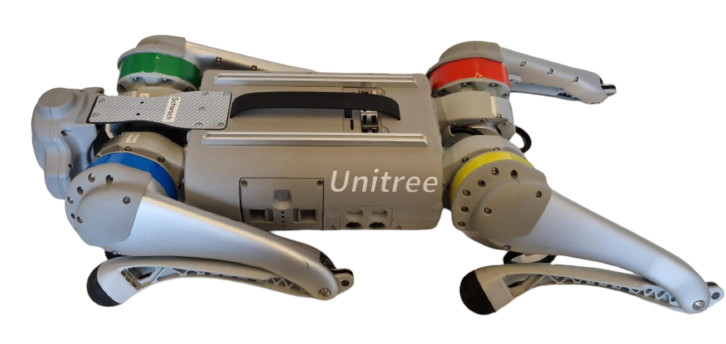
\includegraphics[width=\linewidth]{img/analyse/ausgangsposition}}
    \caption{Ausgangsposition des Roboters}\label{fig:ausgangsposition}
\end{figure}

Durch einfaches Drücken auf dem Knopf neben der Ladeanzeige des Akkus wir der Ladestand über die vier \glspl{led}
angezeigt.
Durch ein sofortiges weiteres Drücken und Halten des Knopfes startet der Roboter.
Dies wird über ein kurzes serielles Aufblinken aller vier \glspl{led} signalisiert.
Zudem sind die Lüfter deutlich zu hören.
Durch dasselbe Verfahren - Drücken gefolgt von zweitem Drücken und Halten des Knopfes neben der Ladeanzeige auf
der Unterseite der Fernbedienung wird auch diese angeschaltet.
Ein einmaliges akustisches Signal ertönt beim Anschalten.
Die Fernbedienung verbindet sich automatisch mit dem Roboter.
Im Werkszustand steht der Roboter nach dem Einschalten nach etwa \num{70} - \num{80} Sekunden auf.
Der Roboter kann nun über die Fernbedienung gesteuert werden.

Zum Ausschalten des \gls{go1} sollte dieser in eine liegende Position (\emph{Prone}-State) und anschließend in den \emph{Damping}-State gebracht werden.
Das wird durch die Tastenkombinationen \texttt{L2+A} und \texttt{L2+B} erreicht.
Danach kann der Akku wie beim Anschalten durch Drücken und erneutes Drücken und Halten ausgeschalten werden.
Die \glspl{led} signalisieren das erfolgreiche Ausschalten und die Lüfter schalten sich aus.
Auch die Fernbedienung kann durch dieses Vorgehen ausgeschalten werden.
Hier signalisieren drei kurze akustische Signale das erfolgreiche Ausschalten.

\subsubsection{Stationäre Inbetriebnahme}
\label{subsubsec:inbetriebnahme_netzteil}

Im Gegensatz zur mobilen Inbetriebnahme wird hier die Inbetriebnahme des Roboters durch eine stetige Stromversorgung durch ein Netzteil
bezeichnet.
Hierfür müssen einige Vorbereitungen getroffen werden, da im Lieferumfang kein Netzteil für den Betrieb des \gls{go1}
enthalten ist.

\begin{requirements}
    \gls{go1}, Netzteil für Akkuladegerät\newline
    \textbf{Zusätzlich:} Hohlstecker M \num{5,5}/\num{2,1} mm auf Schraubklemme, XT30-M Stecker mit ausreichend (> \num{10} cm)
    Verkabelung.
    Alternativ: XT30-M auf Hohlstecker M \num{5,5}/\num{2,1} mm Adapter.
\end{requirements}

Vergleicht man Ausgangsspannung und maximale Stromstärke des verbauten Akkus mit den selben Werten des Netzteils für das
Akkuladegerät, so erkennt man, dass das Ladegerät die passende Ausgangsspannung und Leistung vorweist, um den \gls{go1}
über den in Kapitel \ref{subsubsec:recheneinheiten} Abbildung \ref{fig:vogelperspektive} beschriebenen \emph{XT-30} Port
zu betreiben.
Da das Netzteil lediglich einen Hohlstecker zum Anschluss bietet, muss hierfür jedoch in Eigenarbeit ein Adapter auf XT-30
hergestellt werden.
Herbei sind die in den Ressourcen beschriebenen Bauteile nötig, die Schraubverbindung ist zwar optional und kann durch eine
Lötstelle oder ein vorgefertigtes Teil ersetzt werden, sie erleichtert jedoch die Beschaffung und den Zusammenbau des Adapters.
Zu beachten ist hierbei nur ide korrekte Abmantelung der Kabel für die Schraubklemme und die Orientierung der Kabel in der
Klemme.
Abbildung \ref{fig:xt30} zeigt eine beispielhafte Umsetzung des Beschriebenen und die korrekte Orientierung des XT-30 Steckers.

\begin{figure}[h]
    \frame{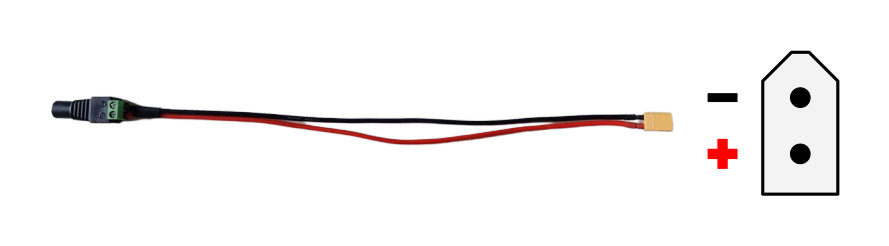
\includegraphics[width=\linewidth]{img/analyse/xt30}}
    \caption{XT-30 auf Hohlstecker Verkabelung und XT-30 Orientierung}\label{fig:xt30}
\end{figure}

Aus Sicherheitsgründen sollte der sogenannte \emph{Sportmodus} des \gls{go1} deaktiviert werden, da sich dieser sonst nach
Start des Roboters aufsteht, was die Verkabelung lösen könnte.
Zudem ist die maximale Ausgangsleistung des Netzteils nicht hoch genug, um den Roboter dauerhaft inklusive der Motoren
zu betreiben.
Der Betrieb wird deshalb stationär genannt.
Für das Deaktivieren des Sportmodus muss sich zunächst auf den Raspberry Pi verbunden werden.
Im Home-Ordner des Nutzers \emph{pi} befindet sich der Ordner \texttt{Unitree/autostart/triggerSport} mit der Datei
\texttt{trig\-ger\-Sport.sh}.
Diese muss lediglich umbenannt werden, beispielsweise zu \texttt{trig\-ger\-Sport.dis\-a\-bled.sh}.

\begin{lstlisting}[language=sh,label=lst:disable-triggersport]
pi@raspberrypi:~ $ cd Unitree/autostart/triggerSport/
pi@raspberrypi:~/Unitree/autostart/triggerSport $ ls
build  log  triggerSport.sh  version.txt
pi@raspberrypi:~/Unitree/autostart/triggerSport $ mv triggerSport.sh triggerSport.disabled.sh
pi@raspberrypi:~/Unitree/autostart/triggerSport $ ls
build  log  triggerSport.disabled.sh  version.txt
\end{lstlisting}

\noindent Beim Neustart des Roboters wird nun nicht automatisch in den Sportmodus geschaltet und die Motoren bewegen sich nicht.
Weiteres zur \emph{Autostart}-Funktion des \gls{go1} in Kapitel \ref{subsubsec:software-autostart}.

Zuletzt kann das Netzteil inklusive des Adapters nun in den XT-30 Port auf dem Rücken des Roboters gesteckt werden.
Ein erfolgreicher Start des Roboters kann über das akustische Wahrnehmen der Lüfter geprüft werden.
Zum Ausschalten muss der Stecker lediglich entfernt und der Roboter somit vom Strom getrennt werden.
Hierfür muss nur sichergestellt sein, dass alle manuellen Operationen auf den Recheneinheiten vollendet sind, damit diese
nicht korrumpiert werden.



\subsection{Hardware Architektur}
\label{subsec:hardware-architektur}

Im folgenden Kapitel wird der Aufbau des intern verbauten Hardware-Systems und die Funktion der einzelnen Bauteile
dessen dargestellt.
Hierfür wird vorerst ein kurzer Überblick über die Komponenten und ihren Zusammenhang geschaffen, was sich in Teilen
mit der Ausführung im vorigen Kapitel \ref{subsubsec:recheneinheiten} überschneidet.
Mit dem geschaffenen Überblick werden die Einzelteile des Systems genauer betrachtet und dokumentiert.
Dies soll über die einfache Dokumentation des Herstellers deutlich hinaus gehen.
Abschließend wird die interne Kommunikation der Bauteile in sich und mit externen Komponenten beschrieben.

\subsubsection{Überblick}
\label{subsubsec:ueberblick_hardware}

Als Einstieg in den Überblick soll veranschaulichend Abbildung \ref{fig:hardware_ueberblick} dienen.
Sie zeigt die einzelnen Komponenten und ihre Verbindungen untereinander und zu den erweiterten Systemen wie dem \gls{bms}
oder der Sensorik.

\begin{figure}[h]
    \frame{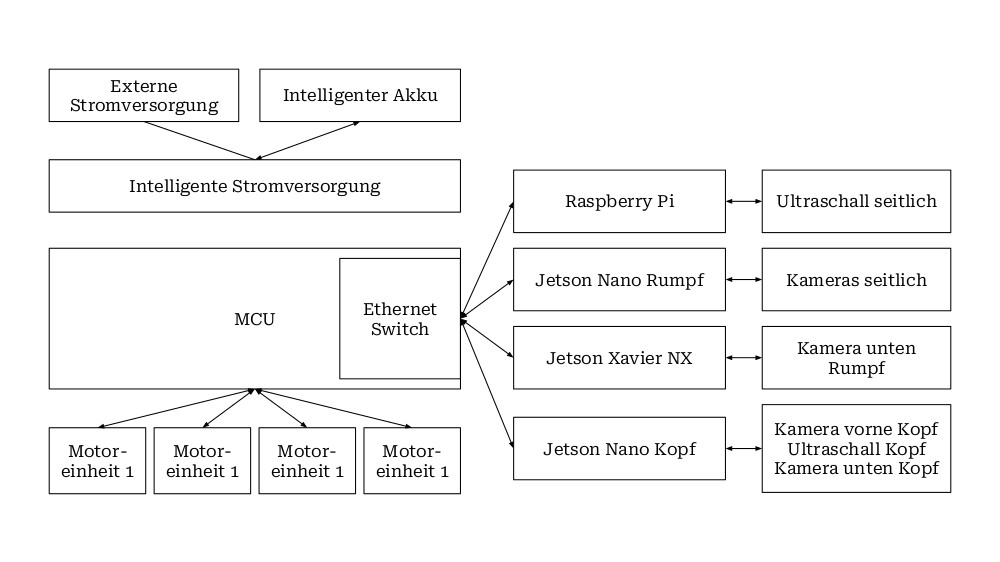
\includegraphics[width=\linewidth]{img/hardware_architektur/ueberblick}}
    \caption{Überblick über die interne Architektur des Go1}\label{fig:hardware_ueberblick}
\end{figure}

Als Grundlage für sowohl die interne Hardware als auch die mechanischen Komponenten dienen die \gls{mcu} und das \gls{bms}.
Beide werden vom Hersteller nicht für den Zugriff freigeschaltet und können lediglich indirekt verwendet werden.
So können beispielsweise die Daten der Motoren und deren Steuerung aktuell nur über Bibliotheken gelesen und manipuliert werden.
Auch die Daten des \gls{bms} sind nur lesend verfügbar.
Zentral zu allen Komponenten steht ein Switch, welcher diese über ein Netzwerk verbindet.
Direkt daran angeschlossen sind alle drei \emph{NVIDIA Jetson} Einheiten - zwei Nanos und ein Xavier NX, der \emph{Raspberry Pi},
die \emph{\gls{mcu}} und der nach außen verfügbar gemachte \emph{RJ-45 Port}.
Der Raspberry Pi kann als zentraler Baustein für alle Entwickler am \gls{go1} bezeichnet werden.
Bis auf dedizierte Auswertungen oder Zugriffe auf die Kameramodule werden die meisten Prozesse zumindest auf dem Pi verwaltet.
Die NVIDIA Einheiten hingegen verarbeiten die ihnen zugeordneten Kameramodule, mit der Ausnahme des Nanos im Kopf des Roboters,
der zudem auch die Sensordaten des nach vorne gerichteten Ultraschallsensors abgreift und verfügbar macht.
Der NVIDIA Jetson Xavier NX ist zudem die rechen-stärkste Einheit mit Blick auf Prozessor und Grafikeinheiten und kann
deshalb im \gls{ml} Bereich und in der Videoauswertung verwendet werden.
Folgende Übersicht zeigt die Verteilung der zugreifbaren Recheneinheiten zu den zu verwaltenden Bausteinen.
\newline

\begin{table}[h]
    \centering
    \begin{tabularx}{\textwidth}{X|X|X|X}
        \textbf{Raspberry Pi} & \textbf{Nano 1 (Kopf)} & \textbf{Nano 2 (Rumpf)} & \textbf{Xavier NX} \\ \hline
        &                        &                         &                    \\
        Wifi Modul            & \gls{led}-Steuerung    & Videoauswertung         & Videoauswertung    \\
        Webhosting            & Audio-Ausgabe          & links + rechts          & Rumpf unten        \\
        App-Verbindung        & Ultraschall frontal    &                         & \gls{ml} Prozesse  \\
        Monitoring            & Videoauswertung        &                         &                    \\
        Bibliotheken          & Kopf vorne/unten       &                         &                    \\
        Ultraschall seitlich  &                        &                         &                    \\
        &                        &                         &
    \end{tabularx}
    \label{tab:ueberblick_hardware_funktionen}
\end{table}

Das nächste Kapitel geht auf Grundlage des Überblicks genauer auf die einzelnen Bausteine der internen Hardware des \gls{go1}
ein.

\subsubsection{Kernelemente}

Als Kernelemente des \gls{go1} werden der verbaute \emph{Raspberry Pi}, die zwei verbauten \emph{NVIDIA Jetson Nanos} und
der \emph{NVIDIA Jetson Xavier NX} bezeichnet.
Grundsätzlich ist die \gls{mcu} ebenfalls als Kernelement zu bezeichnen, sie ist jedoch nicht für den Zugriff durch den
Entwickler freigeschaltet und wird deshalb nicht weiter betrachtet.
Zur genaueren Inspektion der Komponenten kann ein externer Rechner per \emph{Ethernet} an den in Kapitel \ref{subsubsec:recheneinheiten}
\emph{RJ-45}-Port angeschlossen werden.
Diesem Rechner muss dann eine statische \gls{ip}-Adresse im Netz \texttt{192.168.123.0/24} vergeben werden.
Da die \gls{ip}-Adresse noch nicht vergeben sein darf, wurde zur Analyse im Rahmen dieser Arbeit die Adresse \texttt{192.168.123.51}
verwendet.

\myparagraph{Raspberry Pi}
\label{par:raspi}

Laut Hersteller-Dokumentation ist im Roboter ein \emph{Raspberry Pi \num{4}} verbaut.
Anhand der Dokumentation erkennt man lediglich die \gls{ip}-Adresse des Pi - \texttt{192.168.123.161}, jedoch keine Informationen
zu den Eigenschaften dessen.
Zur Prüfung der Eigenschaften des Pis kann sich mit dem Roboter per Ethernet verbunden werden.
Über den Standard-Nutzer kann sich laut Dokumentation per \gls{ssh} auf den Roboter verbunden werden.

\begin{lstlisting}[language=sh,label=lst:pi-ssh]
# user: pi, password: 123, root-password:123
ssh pi@192.168.123.161
\end{lstlisting}

\noindent Als Erstes soll das genaue Modell des Raspberry Pi erkannt werden:

\begin{lstlisting}[language=sh, label=lst:pi-model]
pi@raspberrypi:~ $ grep Model /proc/cpuinfo
Model		: Raspberry Pi Compute Module 4 Rev 1.0
\end{lstlisting}

\noindent Die Prüfung der verbauten Variante des Compute Model 4 lässt dich durch folgendes Kommando durchführen:

\begin{lstlisting}[language=sh, label=lst:pi-ram]
pi@raspberrypi:~ $ grep MemTotal /proc/meminfo
MemTotal:        1894664 kB
\end{lstlisting}

\noindent Eine kurze Prüfung der Herstellerwebsite zeigt uns, dass ein \texttt{Broadcom BCM2711 quad-\allowbreak core Cortex-\allowbreak A72 (ARM v8) 64-bit SoC @ 1.5GHz}
in der Variation mit \num{2} \gls{gb} Arbeitsspeicher verbaut ist.
Die Boot-Partition und der initiale Festplattenspeicher werden bei diversen Kleinplatinenrechner oftmals über eine \gls{sd}-Karte
realisiert.
Um das auf dem Raspberry Pi zu prüfen kann die Belegung des Dateisystems ausgegeben werden.
Die temporären Dateisysteme werden hierbei ausgeschlossen.

\begin{lstlisting}[language=sh, label=lst:pi-sd]
pi@raspberrypi:~ $ df -HTx tmpfs -x devtmpfs
Filesystem     Type  Size  Used Avail Use% Mounted on
/dev/root      ext4   32G   18G   13G  59% /
/dev/mmcblk0p1 vfat  265M   69M  196M  26% /boot
\end{lstlisting}

\noindent Zu erkennen ist, dass tatsächlich eine \gls{sd}-Karte als Boot-Partition unter \texttt{/dev/mmcblk0p1} eingebunden wurde.
Zudem lässt sich die Gesamtgröße des Dateisystems ablesen - \num{32} \gls{gb}.
Zur Prüfung des verbauten Betriebssystems und des Linux Kernels kann folgendes Kommando verwendet werden:

\begin{lstlisting}[language=sh, label=lst:pi-os]
pi@raspberrypi:~ $ grep PRETTY_NAME /etc/os-release
PRETTY_NAME="Debian GNU/Linux 10 (buster)"
pi@raspberrypi:~ $ uname -r
5.4.81-rt45-v8+
\end{lstlisting}

\noindent Zusammenfassend lassen sich die Kerndaten des Pis wie in Tabelle \ref{tab:data-raspi} dargestellt.

\begin{table}[h]
    \centering
    \begin{tabularx}{\textwidth}{|r|X|}
        \hline
        Modell   & Raspberry Pi Compute Module 4 Rev 1.0                              \\ \hline
        SoC      & Broadcom BCM2711 quad-core Cortex-A72 (ARM v8) 64-bit SoC @ 1.5GHz \\ \hline
        RAM      & \num{1894664} kB (\num{1,8} \gls{gb}) Arbeitsspeicher              \\ \hline
        Speicher & \num{32} \gls{gb} Festplattenspeicher über eine \gls{sd}-Karte     \\ \hline
        OS       & Debian 10 (Buster)                                                 \\ \hline
        Kernel   & Linux Kernel 5.4.81-rt45-v8+                                       \\ \hline
    \end{tabularx}\caption{Kenndaten des Raspberry Pi}\label{tab:data-raspi}
\end{table}

Wirft man einen Blick auf die zusätzlich zu den im Raspberry Pi integrierten angeschlossenen Komponenten, so erkennt
man die Funktion des Pi als Schnittstelle zwischen Entwickler und Roboter gut.
Angeschlossene Geräte lassen sich großenteils über die Ausgabe der per \gls{usb} verbundenen Geräte mit dem Befehl
\texttt{lsusb} prüfen.

\begin{lstlisting}[language=sh, label=lst:pi-usb]
pi@raspberrypi:~ $ lsusb
Bus 001 Device 004: ID 0bda:c812 Realtek Semiconductor Corp.
Bus 001 Device 003: ID 2c7c:0125 Quectel Wireless Solutions Co., Ltd. EC25 LTE modem
[...]
\end{lstlisting}

\noindent Nennenswert sind in der Ausgabe besonders der \emph{Realtek} \gls{usb}-WiFi Adapter und das \emph{Quectel}-Modem zum
Einstecken der 4G/ \gls{lte} Karte.
Die genaue Funktion der \gls{usb} Geräte lässt sich oftmals durch eine Suche der Geräteidentifikation links neben dem
vollen Namen des Gerätes auf der Herstellerwebsite prüfen.
Beide Geräte erlauben es dem Pi, sich neben der auf der Platine verbauten Schnittstellen mit dem Internet oder einem lokalen
Netzwerk zu verbinden.

Ein Blick auf die offizielle Dokumentation der Ultraschallsensoren lässt hier erkennen, dass die beiden Sensoren links und rechts
am Rumpf des Roboters über den Serial-Port \texttt{ttyAMA0} verbunden sind.

\begin{lstlisting}[language=sh, label=lst:pi-ultrasonic]
pi@raspberrypi:~ $ dmesg | grep ttyAMA0
[    1.251673] fe201000.serial: ttyAMA0 at MMIO 0xfe201000 (irq = 14, base_baud = 0) is a PL011 rev2
\end{lstlisting}

\noindent Da die Bibliotheken des Herstellers zur Nutzung der Ultraschallsensoren vorkompiliert und nicht dokumentiert ist
konnten über die Verbindungsart und die Nutzung der Sensoren ohne die Bibliothek keine weiteren Informationen gefunden werden.
Dies gilt auch für die Sensoren im Kopf des \gls{go1}.

% --------------------------------------------------------------
% KOPF
\myparagraph{NVIDIA Jetson Nano Kopf}
\label{par:nano-kopf}

Folgt man der Dokumentation der Hersteller, so erreicht man die Recheneinheit im Kopf des Roboters unter der \gls{ip} Adresse \texttt{192.168.123.13}.
Verbinden lässt sich der Rechner über den Nutzer \texttt{unitree} und dem Passwort \texttt{123}.

\begin{lstlisting}[language=sh, label=lst:nanos-ssh]
# user: unitree, password: 123, root disabled
ssh unitree@192.168.123.<nano-ip(13|14|15)>
\end{lstlisting}

Laut Hersteller ist auf allen drei NVIDIA Chips das Betriebssystem Ubuntu installiert, welches auf Debian basiert, aber einige nützliche
Funktionen über die Basis von Debian hinaus mitbringt.
So auch den Befehl \texttt{lshw}, über den sich eine Zusammenfassung der auf dem System verwendeten Hardware ausgeben lässt.

\begin{lstlisting}[language=sh, label=lst:nanos-hardware-kopf, columns=fixed]
unitree@unitree-desktop:~$ sudo lshw -short
[...] Class       Description
[...] =======================
[...] system      NVIDIA Jetson Nano Developer Kit
[...] memory      3962MiB System memory
[...] bridge      NVIDIA Corporation
[...] multimedia  USB2.0 Camera RGB
[...] multimedia  USB2.0 Camera RGB
[...] generic     CP2102N USB to UART Bridge Controller
[...] multimedia  USB Audio Device
\end{lstlisting}

\noindent Erkennbar ist über die gekürzte Ausgabe, dass im Kopf des \gls{go1} ein \emph{NVIDIA Jetson Nano} mit \num{4} \gls{gb}
Arbeitsspeicher verbaut ist.
Zudem sind per \gls{usb} vier externe Geräte angeschlossen, ein Lautsprecher im Rücken des Kopfes, ein Bridge-Controller
zur Steuerung der beiden \gls{led}-Bänder und zwei Kameras.
Die nach vorne gerichtete Kamera ist unter \texttt{/dev/video1} gemountet, die im Kopf nach unten gerichtete Kamera unter
\texttt{/dev/video0}.
Die Dokumentation der Ultraschallsensoren zeigt ebenfalls, dass sich am Serial-Port \texttt{ttyTHS1} der Ultraschall-Sensor
am Kopf des Roboters befindet.

\begin{lstlisting}[language=sh, label=lst:nano-head-ulrtassonic]
unitree@unitree-desktop:~$ dmesg| grep ttyTHS1
[    1.099918] 70006040.serial: ttyTHS1 at MMIO 0x70006040 (irq = 64, base_baud = 0) is a TEGRA_UART
\end{lstlisting}

\noindent Unter den Mountpoints der Kameras können diese ausgelesen und als Quelle verwendet werden.
Ein Blick auf die Dateisysteme zeigt im Gegensatz zum selben Befehl auf dem Raspberry Pi lediglich die \texttt{root}-Partition,
ein weiteres Inspizieren zeigt dann jedoch ebenfalls die \texttt{boot}-Partition auf der \gls{sd}-Karte.

\begin{lstlisting}[language=sh, label=lst:nanos-kopf-fs, columns=fixed]
unitree@unitree-desktop:~$ df -Hx tmpfs -x devtmpfs
Filesystem      Size  Used Avail Use% Mount
/dev/mmcblk0p1   15G   12G  2.5G  83% /

unitree@unitree-desktop:~$ sudo lsblk
NAME         FSTYPE   SIZE MOUNTPOINT
mmcblk0              14.7G
-> mmcblk0p1  ext4     14G /
mmcblk0boot0            4M
mmcblk0boot1            4M
\end{lstlisting}

\noindent Die Prozessorvariante in \texttt{/proc/cpuinfo} gibt \texttt{ARMv8 Processor rev 1 (v8l)} aus.
Ein Blick auf die Herstellerwebsite zeigt, dass mit der Prozessorbezeichnung ein \texttt{Quad-Core ARM Cortex-A57 MPCore} Prozessor verbaut ist\footcite{nvidia_website_vergleich}.
Da die NVIDIA Jetson Reihe auf den Einsatz in der Robotik und im \gls{ml} Bereich optimiert sind, sind neben der \gls{cpu}
starke Grafikeinheiten verbaut.
Laut Hersteller ist eine \texttt{NVIDIA Maxwell-GPU} mit 128 Cores verbaut.
Die genaue Version des Betriebssystems lässt sich analog zum Vorgehen im Raspberry Pi ermitteln:

\begin{lstlisting}[language=sh, label=lst:nanos-kopf-os]
unitree@unitree-desktop:~$ grep PRETTY_NAME /etc/os-release
PRETTY_NAME="Ubuntu 18.04.5 LTS"
unitree@unitree-desktop:~$ uname -r
4.9.201-tegra
\end{lstlisting}

Zusammenfassen lassen sich die Kerndaten des NVIDIA Jetson Nanos im Kopf des Roboters wie in Tabelle \ref{tab:data-head-nano} dargestellt:

\begin{table}[h]
    \centering
    \begin{tabularx}{\textwidth}{|r|X|}
        \hline
        Modell    & NVIDIA Jetson Nano Developer Kit                               \\ \hline
        GPU       & NVIDIA Maxwell-GPU mit 128 Cores                               \\ \hline
        Prozessor & Quad-Core ARM Cortex-A57 MPCore                                \\ \hline
        RAM       & \num{3962} MiB (\num{4} \gls{gb}) Arbeitsspeicher              \\ \hline
        Speicher  & \num{16} \gls{gb} Festplattenspeicher über eine \gls{sd}-Karte \\ \hline
        OS        & Ubuntu 18.04.5 LTS                                             \\ \hline
        Kernel    & 4.9.201-tegra                                                  \\ \hline
    \end{tabularx}\caption{Kenndaten des NVIDIA Jetson Nano im Kopf des Roboters}\label{tab:data-head-nano}
\end{table}


\myparagraph{NVIDIA Jetson Nano Rumpf}
\label{par:nano-rumpf}

Der Nano im Rumpf des Roboters is dem Nano im Kopf des Roboters gegenüber bis auf die angeschlossenen Geräte und seiner
\gls{ip}-Adresse \texttt{192\allowbreak .168\allowbreak .123\allowbreak .14} identisch.
Die Ausgaben für das Betriebssystem in \texttt{/etc/os-release}, der Kernel-Version aus \texttt{uname -r} und der Informationen
zur \gls{sd}-Karte aus \texttt{df -Hx tmpfs -xdevtmpfs} stimmen bei beiden Geräten überein.
Die Unterschiede in der verbundenen Hardware gehen aus folgender Ausgabe hervor:

\begin{lstlisting}[language=sh, label=lst:nanos-hardware-rumpf, columns=fixed]
unitree@unitree-desktop:~$ sudo lshw -short
[...] Class       Description
[...] =======================
[...] system      NVIDIA Jetson Nano Developer Kit
[...] memory      3964MiB System memory
[...] bridge      NVIDIA Corporation
[...] multimedia  USB2.0 Camera RGB
[...] multimedia  USB2.0 Camera RGB
\end{lstlisting}

Ähnlich zum Nano im Kopf des \gls{go1} sind zwei Kameras verbaut, eine Kamera links im Rumpf von hinten betrachtet unter dem Mounting-Point
\texttt{/dev/video1} und eine Kamera rechts im Rumpf unter \texttt{/dev/video0}.
Als Übersicht zu den Kerndaten des Nanos im Rumpf des Roboters kann Tabelle \ref{tab:data-head-nano} verwendet werden.

% ------------------------------------------------
% Xavier NX
\myparagraph{NVIDIA Jetson Xavier NX}
\label{par:nx}

Die zentrale Recheneinheit mit der höchsten Leistung ist der im Rumpf verbaute \emph{NVIDIA Jetson Xavier NX} mit der internen
\gls{ip}-Adresse \texttt{192.168.123.15}.
Auf dem NX ist - wie auf beiden Nanos - das Betriebssystem Ubuntu installiert.
Auch die Kernel-Version ist identisch zu beiden Nanos.

\begin{lstlisting}[language=sh, label=lst:nx-os]
unitree@nx:~$ grep PRETTY_NAME /etc/os-release
PRETTY_NAME="Ubuntu 18.04.5 LTS"
unitree@nx:~$ uname -r
4.9.201-tegra
\end{lstlisting}

Im Wesentlichen unterscheidet der NX sich in seiner Plattform, der Prozessoreinheit und dem verbauten Arbeitsspeicher
von den beiden Nanos.
Folgende Übersicht gibt die Hardwareausstattung aus:

\begin{lstlisting}[language=sh, label=lst:nanos-hardware-rumpf-nx, columns=fixed]
unitree@nx:~$ sudo lshw -short
[sudo] password for unitree:
[...] Class       Description
[...] =======================
[...] system      NVIDIA Jetson Xavier NX Developer Kit
[...] memory      7773MiB System memory
[...] bridge      NVIDIA Corporation
[...] multimedia  USB2.0 Camera RGB
\end{lstlisting}

Laut Hersteller ist im NX ein \texttt{6-Core NVIDIA Carmel ARM v8.2 64-\allowbreak bit-\allowbreak CPU} verbaut\footcite{nvidia_website_vergleich}.
Benchmarks und Vergleiche zu den Recheneinheiten werden in Kapitel \ref{subsec:limitierungen} gezeigt, es kann jedoch
festgehalten werden, dass der NX deutlich fähiger ist, als die beiden Nanos in Kopf und Rumpf.
Zusätzlich zum besseren Prozessor sind im NX \num{8} \gls{gb} Arbeitsspeicher verbaut.
Die angeschlossene Kamera ist die im Rumpf nach unten gerichtete Kamera.
Ein Blick auf die Festplattenkapazitäten des NX stellt auch klar, warum Unitree diese Einheit als Kernstück der Rechenleistung des
\gls{go1} bewirbt.

\begin{lstlisting}[language=sh, label=lst:nx-fs,columns=fixed]
unitree@nx:~$ df -Hx tmpfs -x devtmpfs
Filesystem      Size  Used Avail Use% Mounted on
/dev/nvme0n1p1  118G   22G   90G  20% /
/dev/mmcblk0p1   15G   84M   14G   1% /media/unitree/cd8bfc0a-0f39-4efa-b376-116833b08f45
\end{lstlisting}

Die deutlich höhere Speicherkapazität durch das Anschließen einer \gls{ssd} zusätzlich zur für den Bootvorgang verwendeten
\gls{sd} Karte ermöglicht dem NX das Auswerten größerer Datenmengen als auf den beiden Nanos mit nur \num{16} \gls{gb}
Speicherkapazität auf deren \gls{sd}-Karten.
Wie auf den Nanos ist auch auf dem NX die Grafikeinheit deutlich wichtiger als die Recheneinheit.
Laut Hersteller ist eine \texttt{NVIDIA Volta-GPU} mit 384 Cores und 48 Tensor Cores verbaut.
Auch hier ist der NX deutlich besser ausgestattet als die beiden Nanos.
Tabelle \ref{tab:data-nx} fasst die Eigenschaften des NVIDIA Jetson Xavier NX kurz zusammen.

\begin{table}[h]
    \centering
    \begin{tabularx}{\textwidth}{|r|X|}
        \hline
        Modell    & NVIDIA Jetson Xavier NX                                        \\ \hline
        GPU       & NVIDIA Volta-GPU mit 384 Cores und 48 Tensor Cores             \\ \hline
        Prozessor & 6-Core NVIDIA Carmel ARM v8.2 64-bit-CPU                       \\ \hline
        RAM       & \num{7773} MiB (\num{8} \gls{gb}) Arbeitsspeicher              \\ \hline
        Speicher  & \num{16} \gls{gb} Festplattenspeicher über eine \gls{sd}-Karte \\
        & \num{120} \gls{gb} \gls{ssd} Speicher                          \\ \hline
        OS        & Ubuntu 18.04.5 LTS                                             \\ \hline
        Kernel    & 4.9.201-tegra                                                  \\ \hline
    \end{tabularx}\caption{Kenndaten des NVIDIA Jetson Xavier NX}\label{tab:data-nx}
\end{table}

\todo[inline]{NX Modus 10/15/20W}
% todo NX Modi

\subsubsection{Netzwerk}

Aufgrund der vielen Komponenten, Funktionen und den möglichen Erweiterungen des \gls{go1} ist eine robuste interne Kommunikation nötig.
Die interne Kommunikationsstruktur des Roboters baut großenteils auf Netzwerkstandards wie \emph{Ethernet} und \emph{Wi-Fi} auf,
setzt besonders in der Konnektivität mit externen Komponenten jedoch zusätzlich auf weitere Standards wi \emph{Bluetooth} und \emph{\gls{wwan}}.

Das folgende Kapitel erläutert die vorhandene Kommunikation der internen und externen Komponenten des \gls{go1} und analysiert diese
auf ihre Stärken und Schwächen.
Zudem soll die Methodik der Analyse des Netzwerks und mögliche Problemfeststellungen und -behebungen festgehalten werden.

\subsubsection{Überblick}
\label{subsubsec:netzwerk_ueberblick}

Abbildung~\ref{fig:netzwerk_ueberblick} gilt als Referenz für die folgenden Ausführungen.
Zentrale Einheit der Kommunikation sind der verbaute Ethernet Switch \todo{was für switch} und
der intern verbaute \emph{Raspberry Pi}.
Wie auf Abbildung~\ref{fig:netzwerk_ueberblick} zu erkennen ist, sind alle fünf manipulierbaren Platinen -
der Raspberry Pi, die \gls{mcu}, die beiden Nvidia Jetson Nanos mit \num{4}GB \gls{ram} und der Nano im Kopf des Hundes -
per \emph{Ethernet} mit dem Switch verbunden.
Auch der extern zugängliche Ethernet-Port auf dem Rücken des Roboters ist mit dem Switch verbunden.

\begin{figure}[h]
    \frame{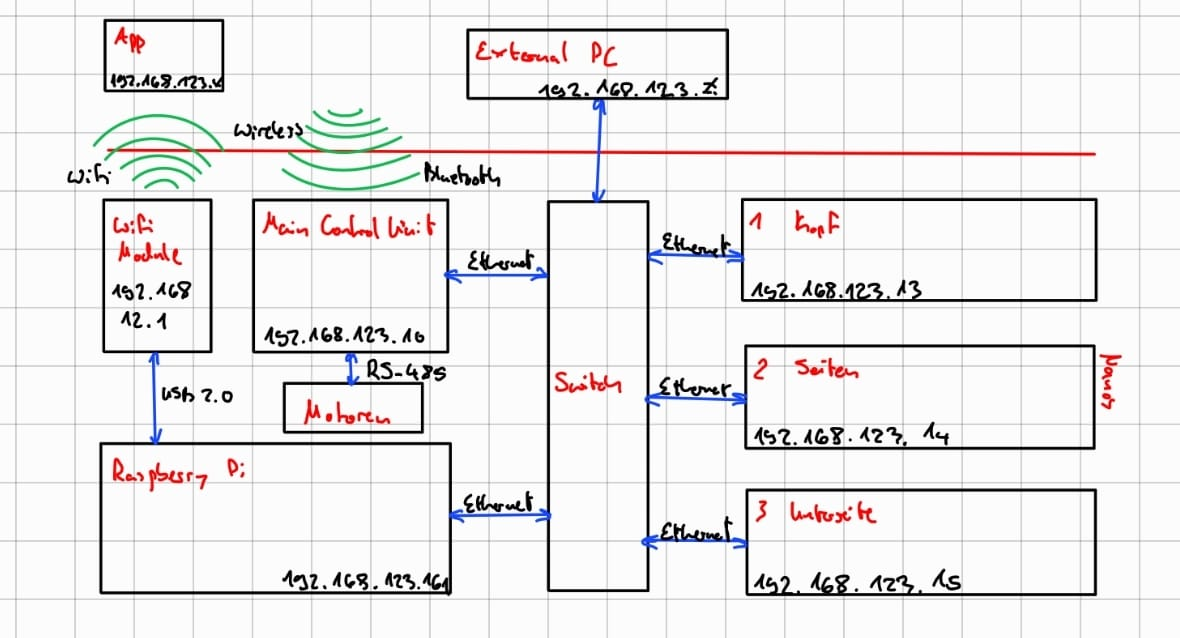
\includegraphics[width=\linewidth]{img/netzwerk/netzwerk_ueberblick}}
    \caption{Überblick über Netzwerkkonfiguration}\label{fig:netzwerk_ueberblick}
\end{figure}\todo{Überblick Quelle aus Anleitung}

Alle geswitchten Komponenten des Netzwerks sind im \texttt{192.168.123.0/24}-Netzwerk registriert.
\todo{was ist gateway? nötig?}
Dabei ist die Verteilung der \gls{ip}-Adressen folgendermaßen vorkonfiguriert:
\begin{itemize}
    \item \textbf{\gls{mcu}:} \texttt{192.168.123.10}
    \item \textbf{Raspberry Pi:} \texttt{192.168.123.10}
    \item \textbf{Nvidia Jetson Nanos:}
    \begin{enumerate}
        \item Kopf: \texttt{192.168.123.13}
        \item Seiten: \texttt{192.168.123.14}
        \item Unterseite: \texttt{192.168.123.15}
    \end{enumerate}
\end{itemize}
Dem Endgerät, das am externen Ethernet-Port an der Oberseite des Roboters angesteckt werden kann,
muss eine statische \gls{ip}-Adresse im Bereich \texttt{192.168.123.0/24} vergeben werden, die nicht bereits von einem der oben genannten
Geräten verwendet wird.

Der Raspberry Pi hat zusätzlich zu seiner physischen Verbindung zum Switch und der \texttt{192.168.123.161}-\gls{ip}-Addresse
noch ein \gls{wwan} Modul verbaut, mit welchem er das Netz \texttt{192.168.12.0/24} publiziert.
Dieses Netz wird ab Werk für die Verbindung der App mit dem System benötigt.
Dazu mehr in Kapitel \ref{subsubsec:app_and_web}.
Des Weiteren kann dieses Netz genutzt werden, um eine kabellose Verbindung mit dem Gesamtsystem
des Roboters herzustellen.
Hierzu mehr in Kapitel \ref{par:raspi}.

\todo{MCU und Bluetooth? Wie?}
\todo{Welche Art Netzwerk, switched, routed, hub?}






\subsection{Limitierungen}
\label{subsec:limitierungen}

\subsubsection{Rechenleistung}
\subsubsection{Physische Limitierungen}

\todo[inline]{Throttling!}
% Akkulaufzeiten noch einmal messen?